%\documentclass[aspectratio=34]{beamer}
\documentclass{beamer}

% Remove the gratuituous footer
\setbeamertemplate{footline}{}
\setbeamertemplate{navigation symbols}{}
%\renewcommand{\insertnavigation}[1]{}

\usepackage{rotating}
\usepackage{subfigure}
\usepackage{algorithm}
\usepackage{algorithmicx}
\usepackage{algpseudocode}
\usepackage{xcolor}

\usepackage{graphicx}
\DeclareMathOperator{\conv}{conv}
\DeclareMathOperator{\st}{s.t.}
\DeclareMathOperator{\dom}{dom}
\DeclareMathOperator{\im}{im}
\DeclareMathOperator{\Ne}{Ne}
\DeclareMathOperator{\sign}{sign}
\DeclareMathOperator{\Var}{Var}
\DeclareMathOperator{\diag}{diag}
\DeclareMathOperator{\vvec}{vec}


%\usepackage{beamerthemesplit}

% Make footnotes visible. Stolen from http://tex.stackexchange.com/questions/5852/beamer-footnote-text-collides-with-navigation-symbols
\addtobeamertemplate{footnote}{\vspace{-6pt}\advance\hsize-0.5cm}{\vspace{6pt}}
\makeatletter
% Alternative A: footnote rule
\renewcommand*{\footnoterule}{\kern -3pt \hrule \@width 2in \kern 8.6pt}
% Alternative B: no footnote rule
% \renewcommand*{\footnoterule}{\kern 6pt}
\makeatother

\setbeamertemplate{bibliography item}{}
\usepackage[style=authoryear-comp,firstinits,doi=true,isbn=false,url=false,eprint=false,backend=biber]{biblatex}
%\usepackage[sorting=none,firstinits,doi=false,isbn=false,url=false,backend=biber]{biblatex}
\bibliography{ML}
% Don't display series
\AtEveryBibitem{\clearlist{series}}
\AtEveryBibitem{\clearfield{series}}
\DeclareSourcemap{
  \maps[datatype=bibtex]{
    \map{
       \step[fieldset=series, null]
    }
  }
}

\DeclareFieldFormat{titlecase}{\MakeTitleCase{#1}}

% Correct casing for journal titles.
\newrobustcmd{\MakeTitleCase}[1]{%
  \ifthenelse{\ifcurrentfield{booktitle}\OR\ifcurrentfield{booksubtitle}%
    \OR\ifcurrentfield{maintitle}\OR\ifcurrentfield{mainsubtitle}%
    \OR\ifcurrentfield{journaltitle}\OR\ifcurrentfield{journalsubtitle}%
    \OR\ifcurrentfield{issuetitle}\OR\ifcurrentfield{issuesubtitle}%
    \OR\ifentrytype{book}\OR\ifentrytype{mvbook}\OR\ifentrytype{bookinbook}%
    \OR\ifentrytype{booklet}\OR\ifentrytype{suppbook}%
    \OR\ifentrytype{collection}\OR\ifentrytype{mvcollection}%
    \OR\ifentrytype{suppcollection}\OR\ifentrytype{manual}%
    \OR\ifentrytype{periodical}\OR\ifentrytype{suppperiodical}%
    \OR\ifentrytype{proceedings}\OR\ifentrytype{mvproceedings}%
    \OR\ifentrytype{reference}\OR\ifentrytype{mvreference}%
    \OR\ifentrytype{report}\OR\ifentrytype{thesis}}
    {#1}
{\MakeSentenceCase{#1}}}

%%%%%%%%%%%%%%%%%%%%%%%%%%%%%%%%%%%%%%%%%%%%%%%%%%%%%%%%%%%%%%%%%%%%
%% THE ACTUAL DOCUMENT BEGINS
%%%%%%%%%%%%%%%%%%%%%%%%%%%%%%%%%%%%%%%%%%%%%%%%%%%%%%%%%%%%%%%%%%%%

\title{Topic Models for Texts and Images in Representation Space}
\author{Kui Tang and Sameer Lal}
\institute{Columbia University}

\date{18 February 2015}

\begin{document}

\frame{\titlepage}

\begin{frame}
  \frametitle{Topic Models}
  {\centering 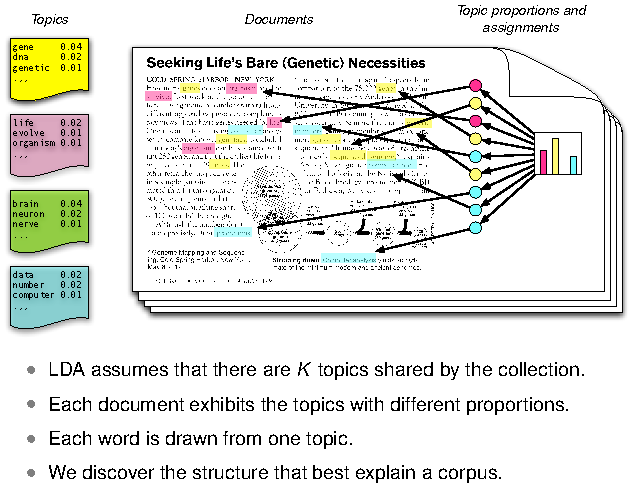
\includegraphics[width=\textwidth]{assets/lda_colors.pdf}}
  {\small \emph{Slide stolen from D. Blei.} \par}
\end{frame}

\begin{frame}
  \frametitle{Latent Variable Models}
  {\centering 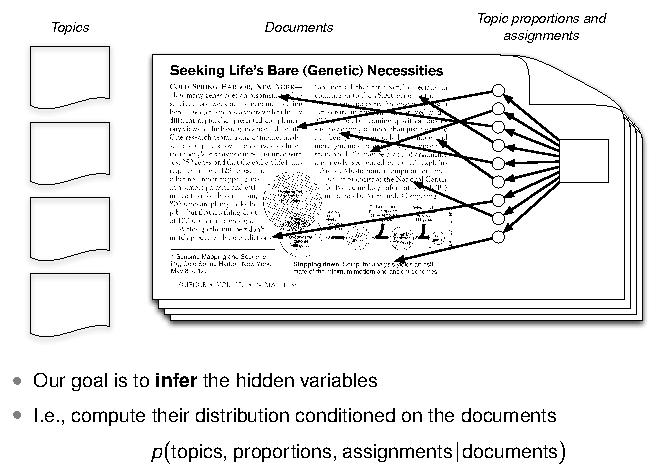
\includegraphics[width=\textwidth]{assets/lda_hidden.pdf}}
  {\small \emph{Slide stolen from D. Blei.} \par}
\end{frame}

\begin{frame}
  \frametitle{Bayesian Networks}
  {\centering 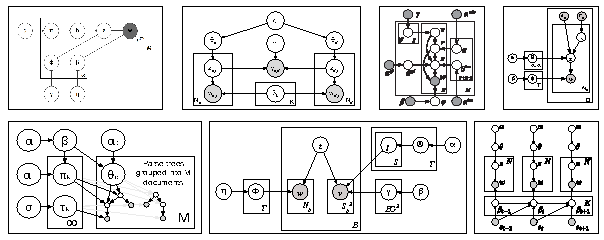
\includegraphics[width=\textwidth]{assets/lda_crazy.pdf}}
  {\small \emph{Slide stolen from D. Blei.} \par}
  \begin{itemize}
  \item Shaded variables are \emph{observed}, other variables are \emph{hidden}.
  \item A model is our hypothesis for how data are generated.
  \item We \emph{condition} on observations to update our hypothesis.
  \end{itemize}
\end{frame}


\begin{frame}
  \frametitle{Multimodal Documents}
  \begin{center}
    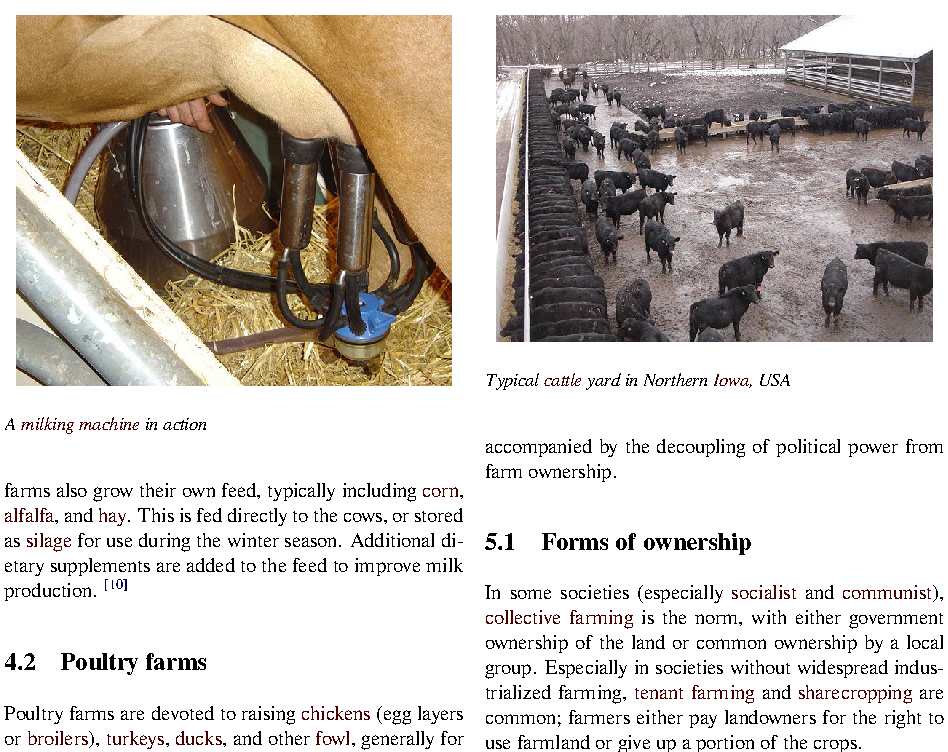
\includegraphics[width=0.75\textwidth]{assets/wiki_farm.pdf}
  \end{center}
             
  \begin{itemize}
  \item \emph{We want to learn a topic model using text and images jointly.}
  \item Images and text complement each other.
  \item Captions aren't the whole story: cows in political contexts.
  \end{itemize}
             
\end{frame}

\begin{frame}
  \frametitle{Gaussian Topic Models with CNNs}
  \begin{center}
    \includegraphics[width=\textwidth]{gtm_cnn.pdf}
    \begin{itemize}
    \item Topics are (mixtures of) Gaussians.
    \item Words are latent vectors $\lambda_v \in \mathbb{R}^{D_W}$ using Bayesian word2vec.
    \item Images are latent vectors $v_{in} \in \mathbb{R}^{D_I}$ where $v_{ni} \sim \mathcal{N}(M \text{cnn}(I_{ni} ; \Omega))$ with $\Omega$ CNN parameters, $M$ mapping to word vector space, and $\text{cnn}$ feature representation output by CNN.
    \end{itemize}
  \end{center}
\end{frame}

\begin{frame}
  \frametitle{Algorithm}
  \begin{algorithm}[H]
      \caption{Frank-Wolfe Algorithm for MLE}
    \begin{algorithmic}
      \State Let $t := 0$, $\tau$ be the uniform distribution, $h(\tau)$ the objective function of the previous slide.
      \Repeat
        \State Compute gradient $g_t := \nabla h(\tau_t)$
        \For{$m := 1:M$}
          \State Find the MAP assignment for the $m$th example $$\tau_{t}^{*(m)}:=\min_{\tau^{(m)}\in{\cal M}}\left\langle g^{(m)}_t,\tau^{(m)}\right\rangle$$
        \EndFor
        \State Linesearch: Find $\eta^{*}$ to minimize $h((1 - \eta)\tau_t + \eta\tau_{t}^{*})$
        \State Update $\tau_{t+1} := (1 - \eta^{*})\tau_t + \eta^{*}\tau_{t}^{*}$
      \Until{duality gap $< \epsilon$} \Comment{Gap converges at rate $O(1/t)$}
    \end{algorithmic}
  \end{algorithm}
  Inner loop can be parallel, or block-coordinate (randomly pick one sample).
\end{frame}

\begin{frame}
  \frametitle{Results on Linear CRFs (Test Error)}
\end{frame}

\begin{frame}
  \frametitle{Results on Linear CRFs (Objective Value)}
\end{frame}

\begin{frame}
  \frametitle{Why Do We Want to Do This?}
  \begin{itemize}
  \item Constructing an unsupervised, non-discrimantive, model
  \item Difficult to measure performance - (Evaluating Topic Models Citation)
  \item Unspervised data can lead to better vector construction
  \item "...in general capture some distributional syntatic and semantic information." (Socher paper citation)
  \item Can this lead to a semantic understanding of multimodal data?
  \end{itemize}
\end{frame}

\begin{frame}
  \frametitle{Related Methods}
  \begin{itemize}
  \item Use Deep Boltzmann Machines - (Srivastava Citation)
  \item Semi-supervised learning for effective generalization from smaller data sets - (Kingma citation)
  \item Deep Visual-Semantic Embedding Model, use both unannotated text and trained image data for classification - (DeViSE Citation)
  \end{itemize}
\end{frame}

\begin{frame}
  \frametitle{Implementation and Applications}
  \begin{itemize}
  \item Image and text modalities: corpa with images, annotated images, images with captions
  \item Code EM algorithm with pretrained Caffe model and custom objective, compare with performing SGD on CNN and variational parameters jointly
  \item Explore other applications: modeling sub-topics, generalization to tangential classes, or image queries and search
  \item Maybe other modalities such as genomics or natural language?
  \item Compare with other algorithms
  \end{itemize}
\end{frame}

\begin{frame}
  \frametitle{Thank You}
  \begin{itemize}
  \item Questions?
  \end{itemize}
\end

\section{References}
\begin{frame}[t,allowframebreaks]{}
\frametitle{References}
\printbibliography
\end{frame}

\end{document}

